\documentclass[10pt, graphics, aspectratio=169, table]{beamer}
\usepackage{hyperref}
\usepackage{booktabs}
\usepackage[normalem]{ulem}
\usepackage[flushleft]{threeparttable}

% -- Change to this year's color! --
\definecolor{ese}{RGB}{58, 240, 212}
\newcommand{\ra}{$\Rightarrow$\ }

\usetheme{metropolis}
\setbeamercolor{frametitle}{bg=ese}

\title{Computer Hardware - A Short Guide}
\author{Armin Wolf}
\date{ESE \the\year{}}
\institute{Nerd::101 - ESE - ifsr - TU Dresden}
\titlegraphic{\hfill
\includegraphics[height=2cm]{../logo}}

\begin{document}
    \maketitle

    \begin{frame}{Outline}
        \tableofcontents
    \end{frame}


    \section{Introduction}
    \begin{frame}{Components of a modern (Desktop) PC}
        \begin{columns}
            \column{0.55\textwidth}
            	We will focus on:
                \begin{itemize}
                    \item Power supply (\textbf{PSU})
                    \item Storage (\textbf{HDD} and \textbf{SSD})
                    \item Graphics card (\textbf{GPU})
                    \item Memory (\textbf{RAM})
                    \item Processor (\textbf{CPU})
                    \item Mainboard
                \end{itemize}
                \textbf{There are many more components, but those are usually the most important ones!}
            \column{0.45\textwidth}
                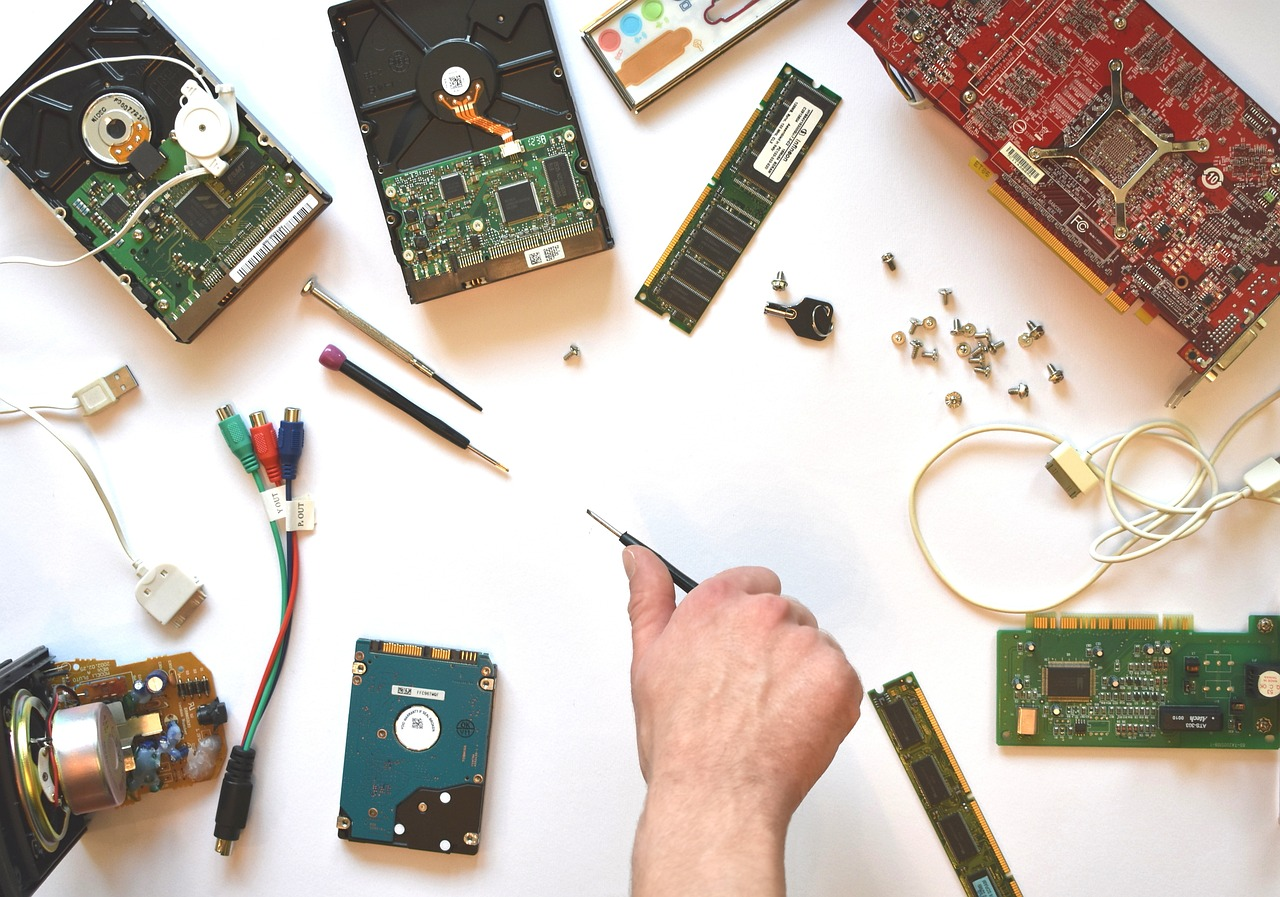
\includegraphics[width=\textwidth]{img/hardware.jpg}
                \center\tiny\url{https://cdn.pixabay.com/photo/2018/07/01/16/52/hardware-3509891_960_720.jpg}
        \end{columns}
    \end{frame}

	\section{Components}
	\begin{frame}{Power Supply}
        \begin{columns}
            \column{0.55\textwidth}
                \begin{itemize}
                	\item \textbf{P}ower \textbf{S}upply \textbf{U}nit
                    \item supplies other components with power
                    \item different efficiency classes \ra better efficiency means less wasted energy
                    \item wide repertoire of connectors (Molex, SATA, ATX, CPU, \ldots)
                    \item physical dimensions standardized \ra easier installation
                \end{itemize}
            \column{0.45\textwidth}
                \center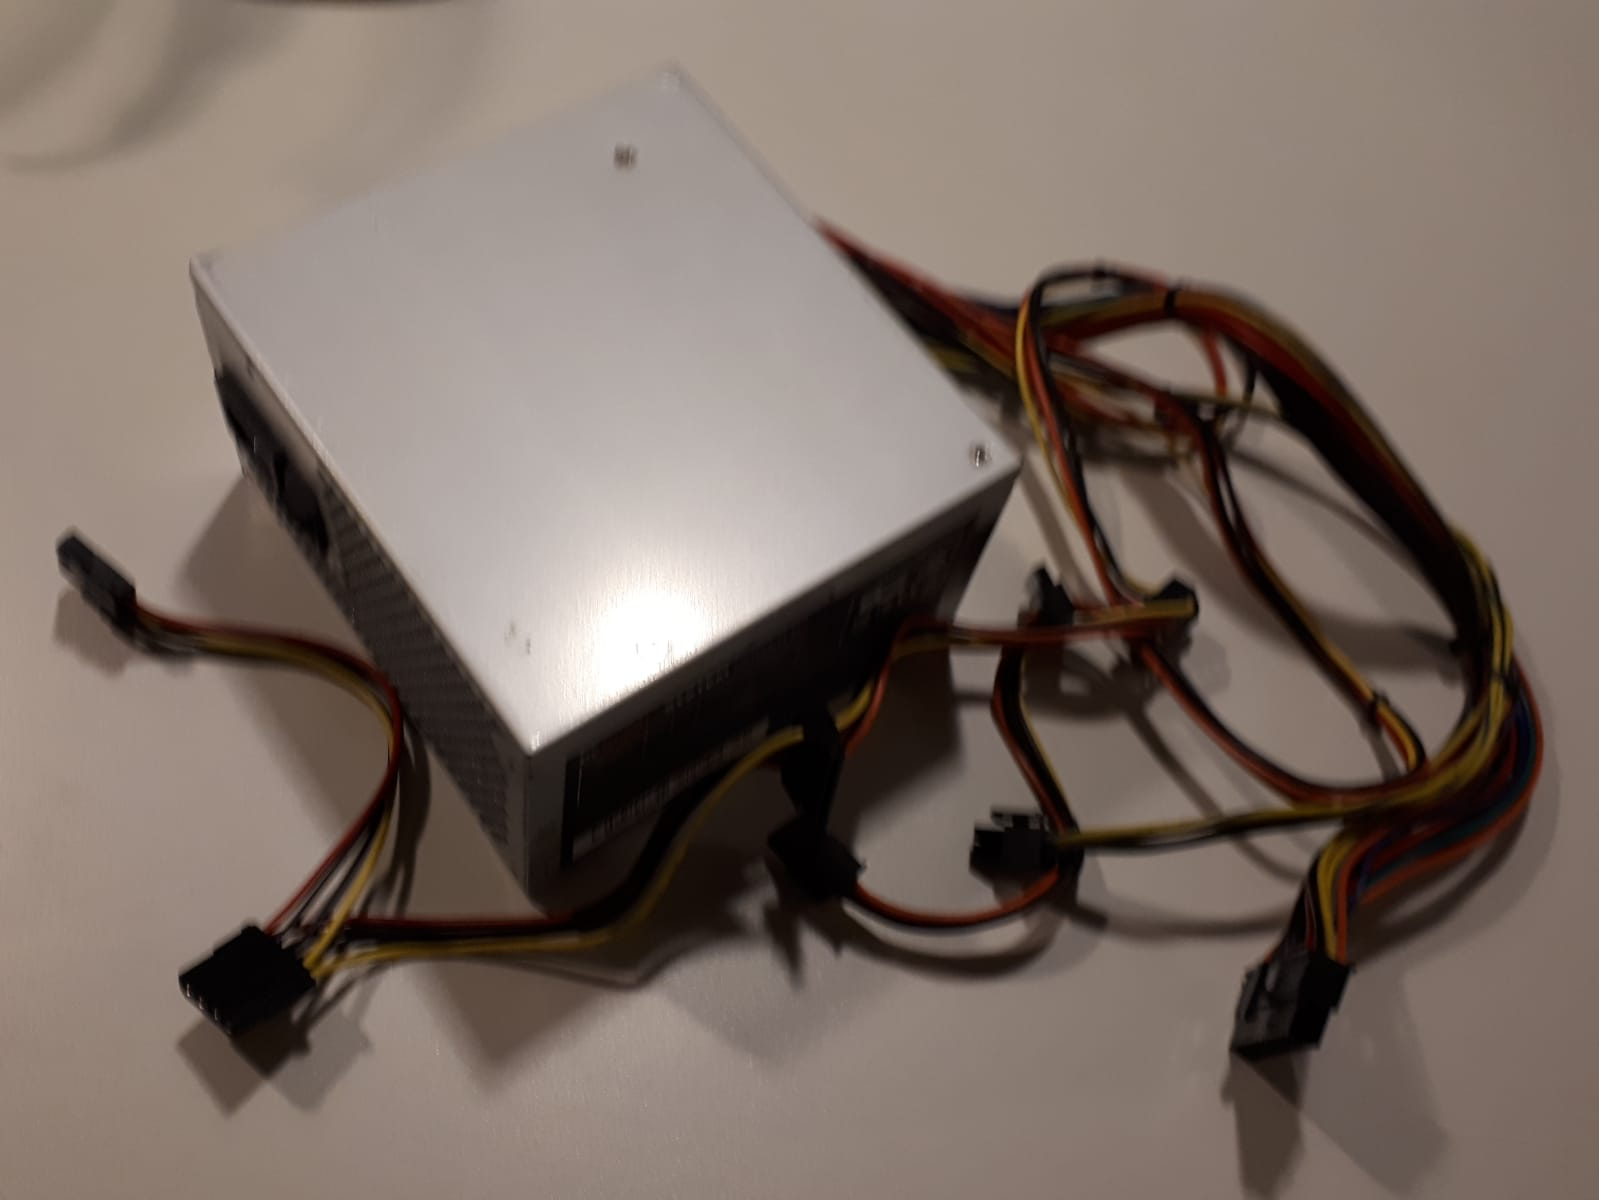
\includegraphics[scale=0.1]{img/psu.jpeg}
        \end{columns}
    \end{frame}
    
    \begin{frame}{Storage}
        \begin{columns}
            \column{0.55\textwidth}
                \begin{itemize}
                    \item \textbf{H}ard \textbf{D}isc or \textbf{S}olid \textbf{S}tate \textbf{D}rive
                    \item stores persistent information
                    \item connected over SATA (cable) or NVMe (extension card)
                    \item physical dimensions are standardized \ra easier installation
                \end{itemize}
            \column{0.45\textwidth}
                \center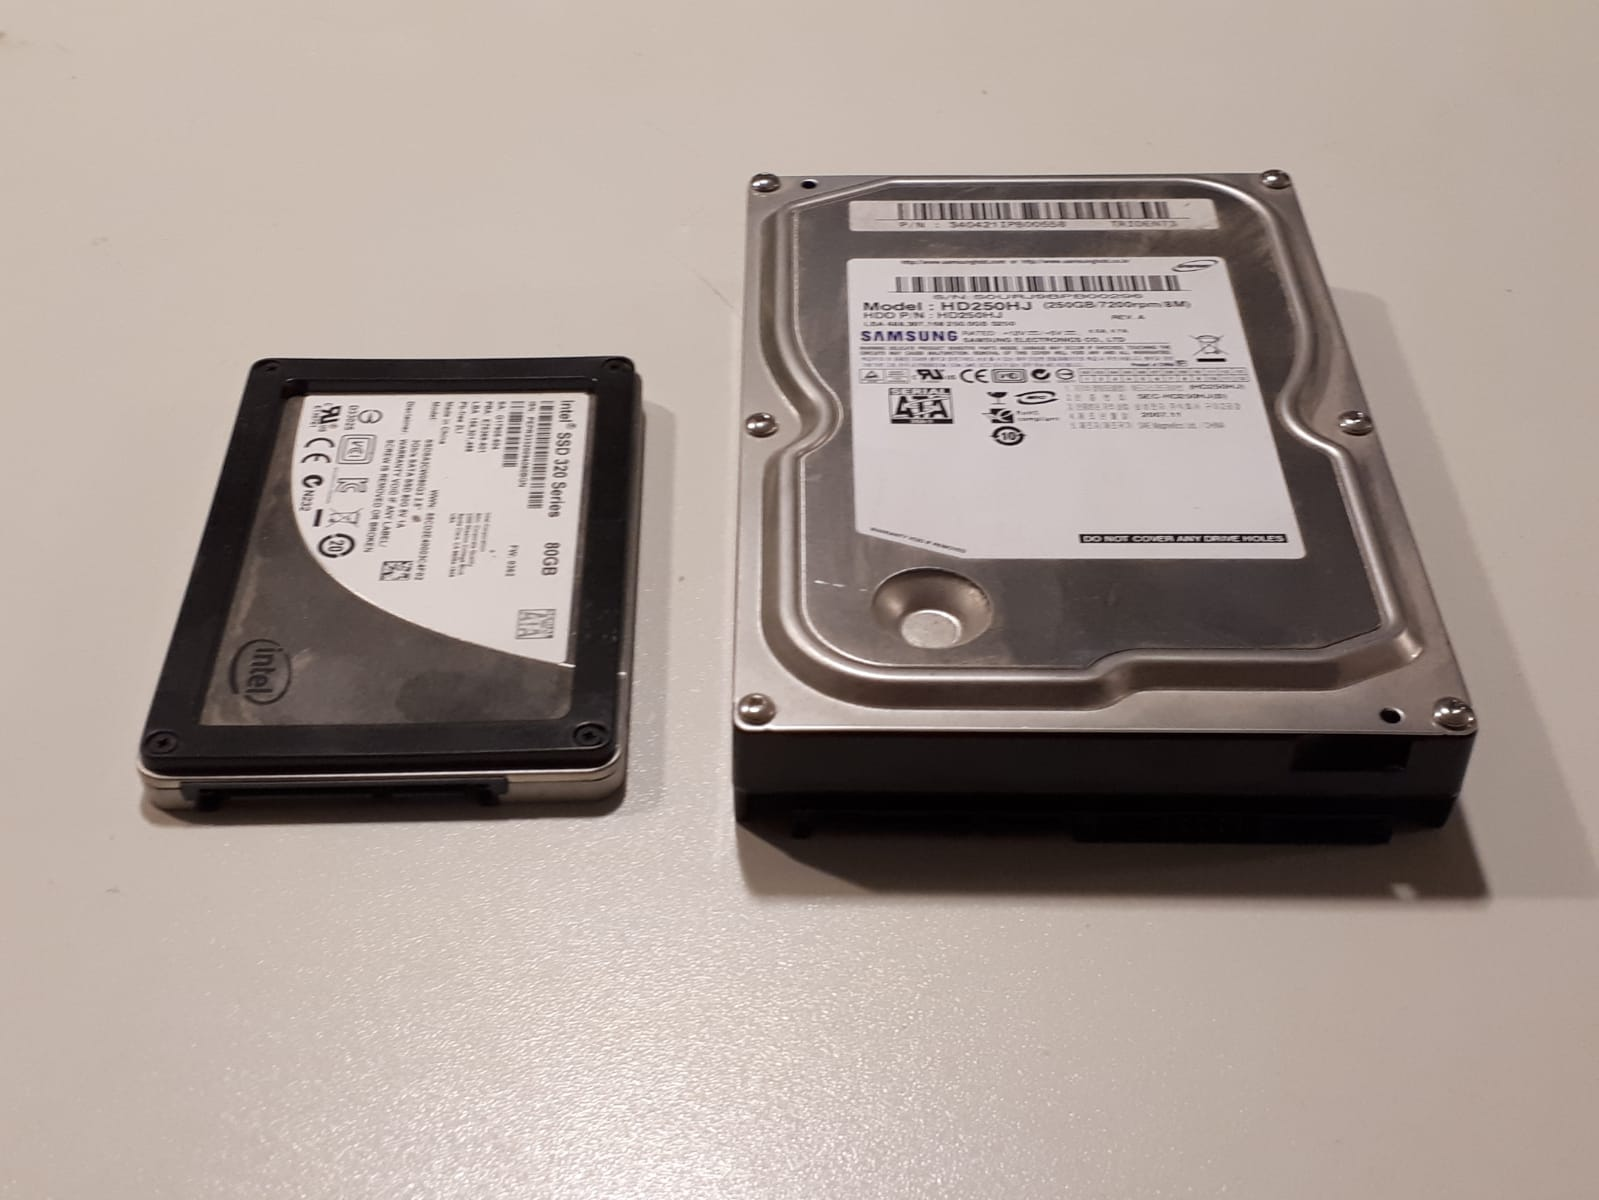
\includegraphics[scale=0.1]{img/hdd_ssd.jpeg}
        \end{columns}
    \end{frame}


    \begin{frame}{Graphics Card}
        \begin{columns}
            \column{0.55\textwidth}
                \begin{itemize}
                	\item \textbf{G}aphics \textbf{P}rocessing \textbf{U}nit
                    \item responsible for handling graphics and related calculations
                    \item available as extension card or integrated inside the processor
                    \item high power consumption \ra additional power cords are sometimes required
                    \item bigger cards are more difficult to install and might not fit inside the computer case
                \end{itemize}
            \column{0.45\textwidth}
                \center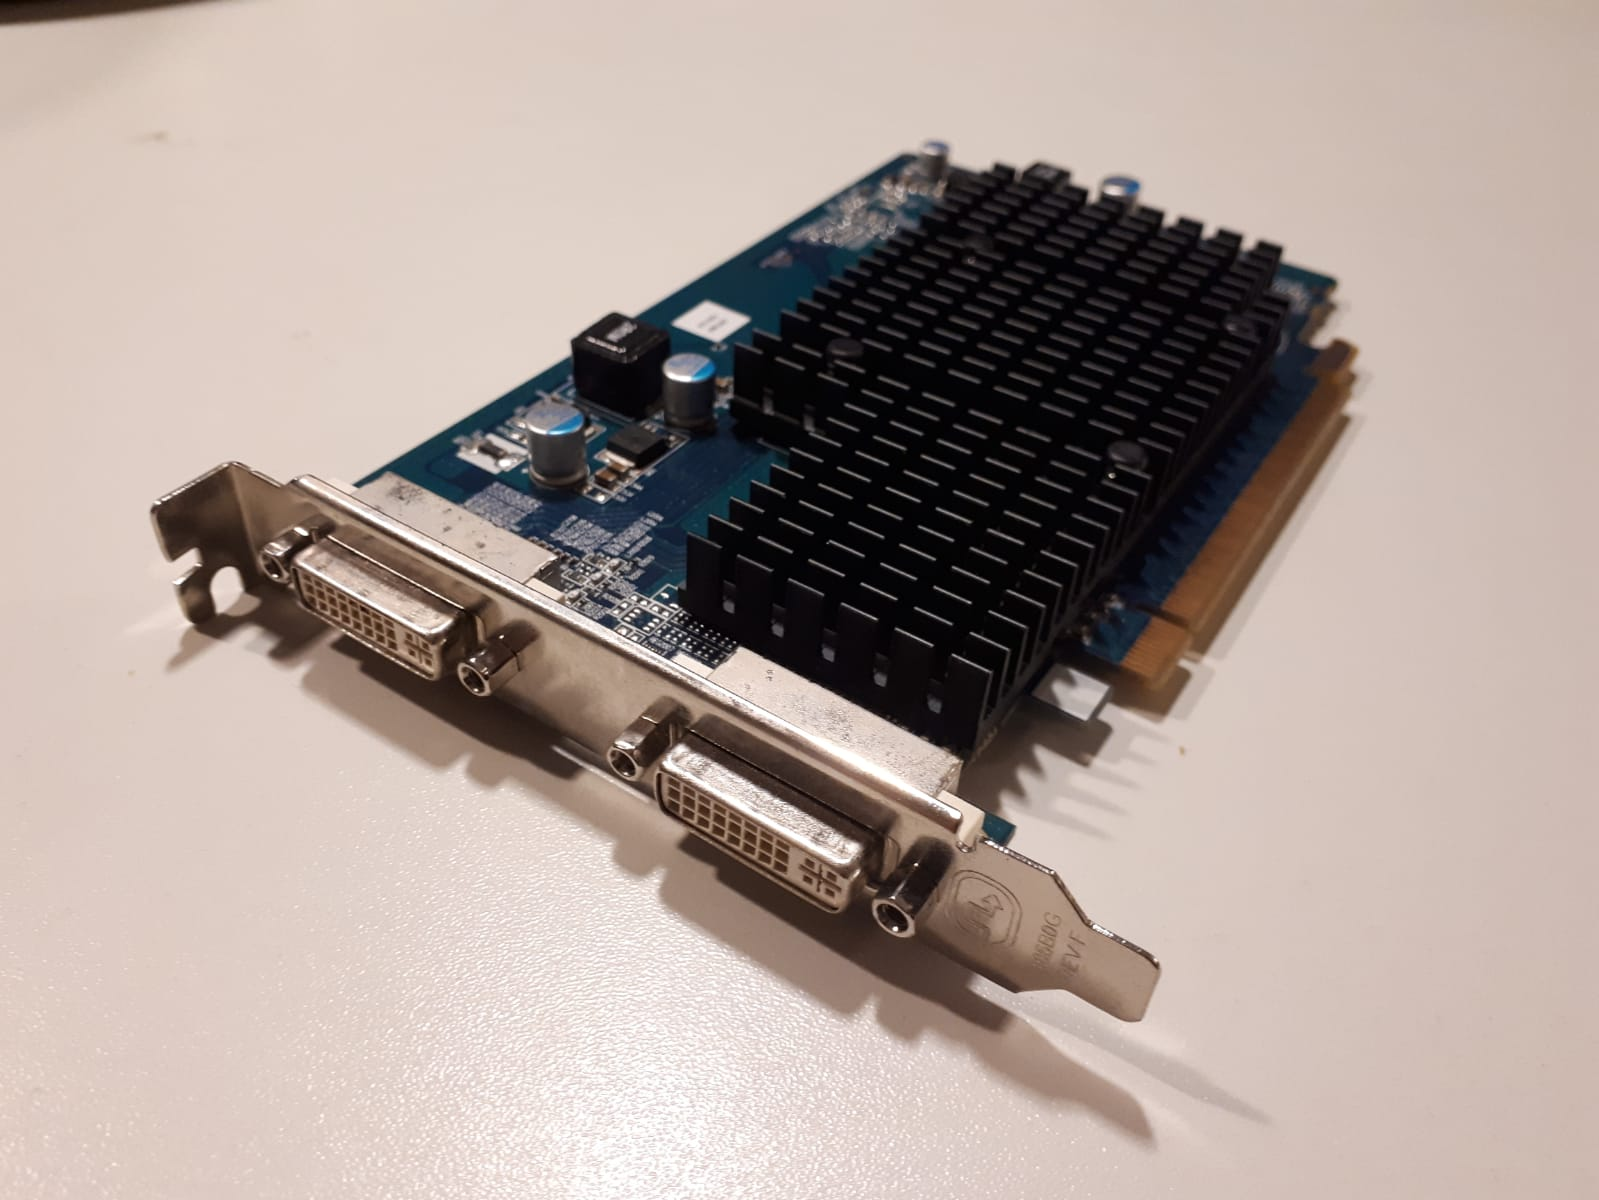
\includegraphics[scale=0.1]{img/gpu.jpeg}
        \end{columns}
    \end{frame}

    \begin{frame}{Memory}
        \begin{columns}
            \column{0.55\textwidth}
                \begin{itemize}
                    \item \textbf{R}andom \textbf{A}ccess \textbf{M}emory
                    \item stores runtime information
                    \item available as memory modules
                    \item different generations available, all incompatible with each other \ra supported generation depends on mainboard model
                    \item installation similar to extension cards, except for a small notch used to prevent installation of incompatible modules
                \end{itemize}
            \column{0.45\textwidth}
                \center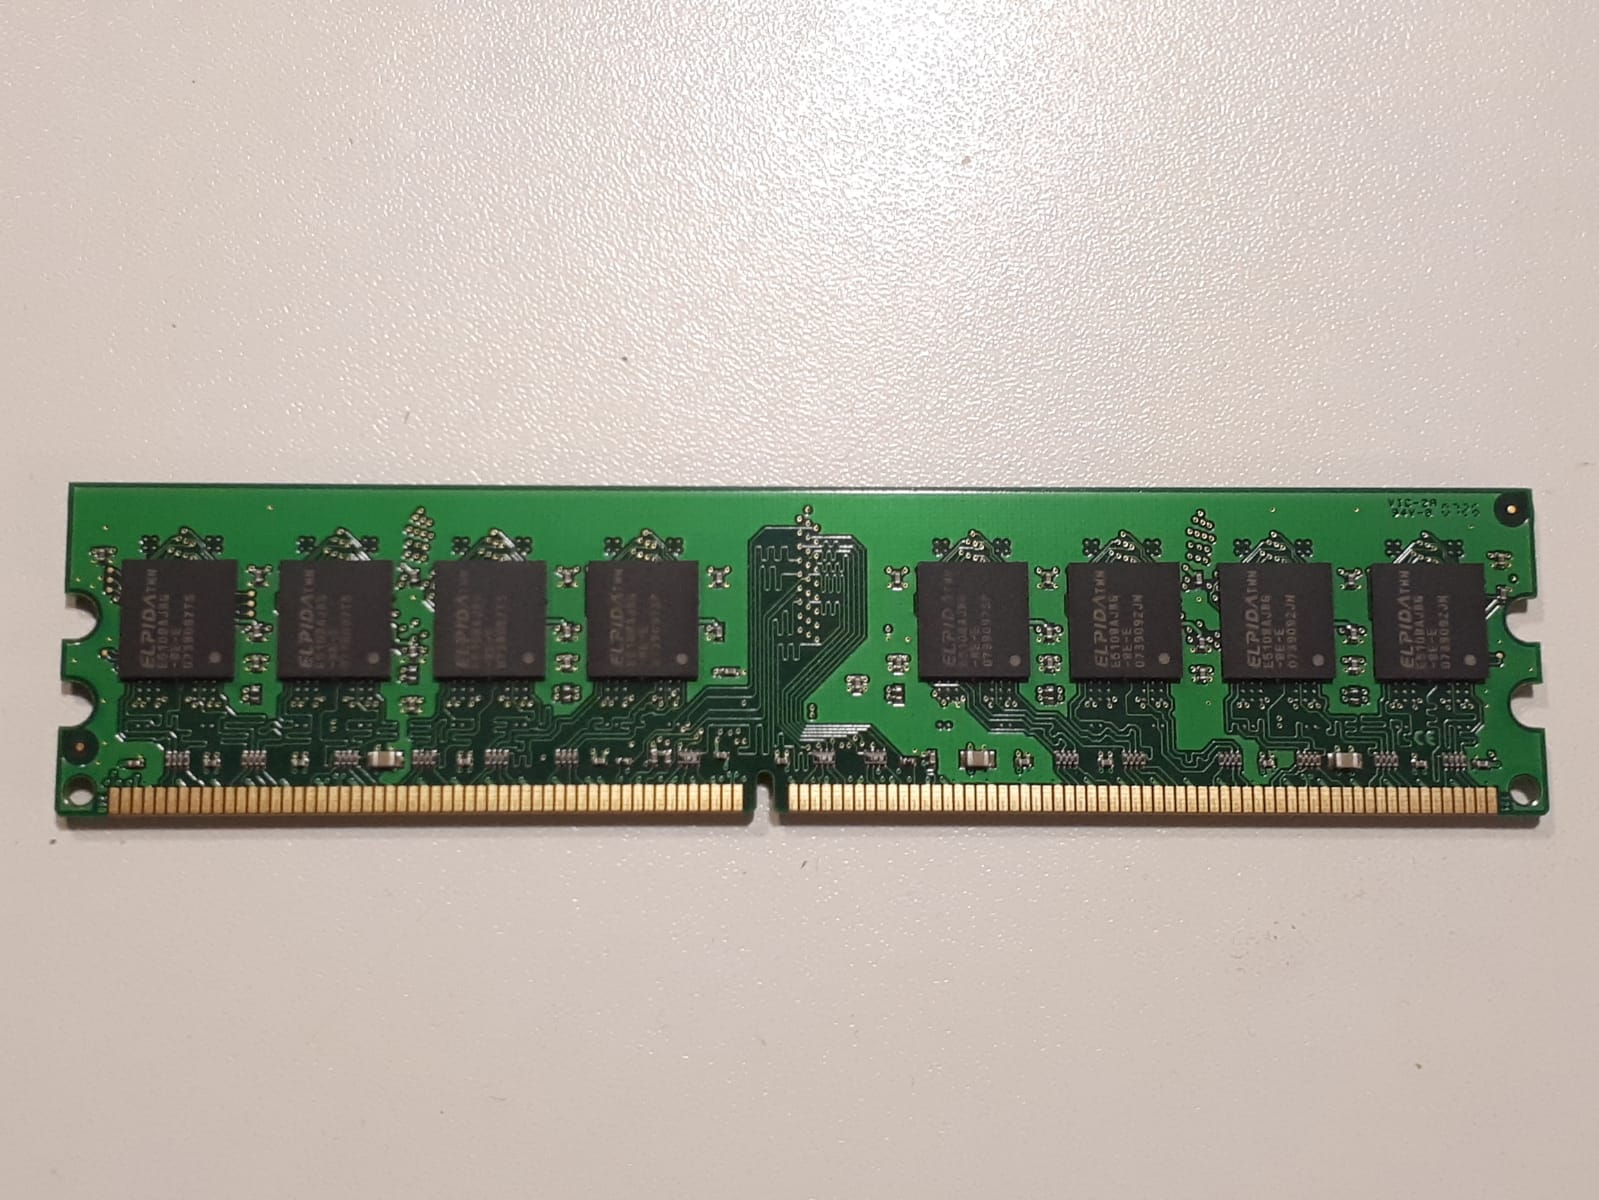
\includegraphics[scale=0.1]{img/ram.jpeg}
        \end{columns}
    \end{frame}
    
    \begin{frame}{Processor}
        \begin{columns}
            \column{0.55\textwidth}
                \begin{itemize}
                	\item \textbf{C}entral \textbf{P}rocessing \textbf{U}nit
                    \item executes programs \ra "brain" of the computer
                    \item needs a dedicated heat sink, together with thermal paste
                    \item connected with the mainboard thru a special socket \ra compatibility depends on mainboard model
                    \item small notches on the sides prevent wrong installation
                \end{itemize}
            \column{0.45\textwidth}
                \center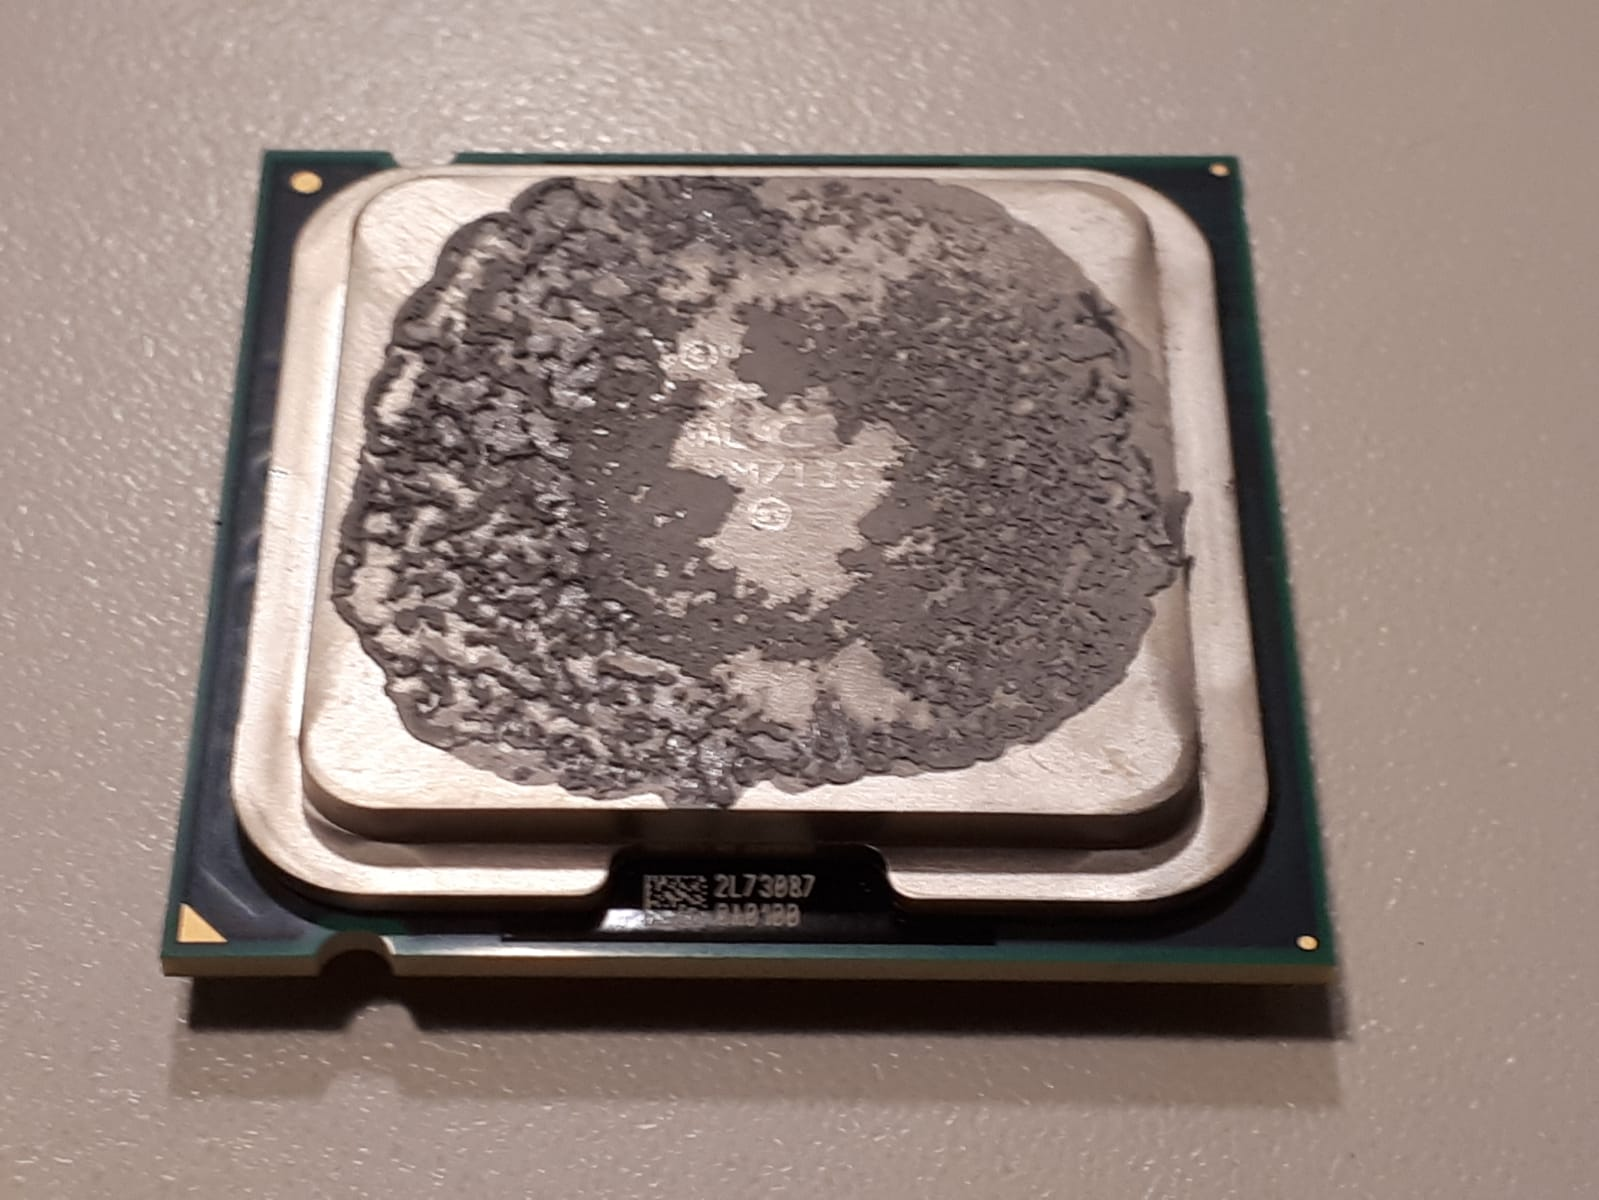
\includegraphics[scale=0.1]{img/cpu.jpeg}
        \end{columns}
    \end{frame}

    \begin{frame}{Mainboard}
        \begin{columns}
            \column{0.55\textwidth}
                \begin{itemize}
                    \item contains the connectors for all the external components plus some onboard devices
                    \item determines supported processors and memory modules
                    \item also handles power distribution
                    \item format \(ATX\) is standardized \ra usually fits inside all computer cases
                    \item directly connected to the computer case using standardized screws
                \end{itemize}
            \column{0.45\textwidth}
                \center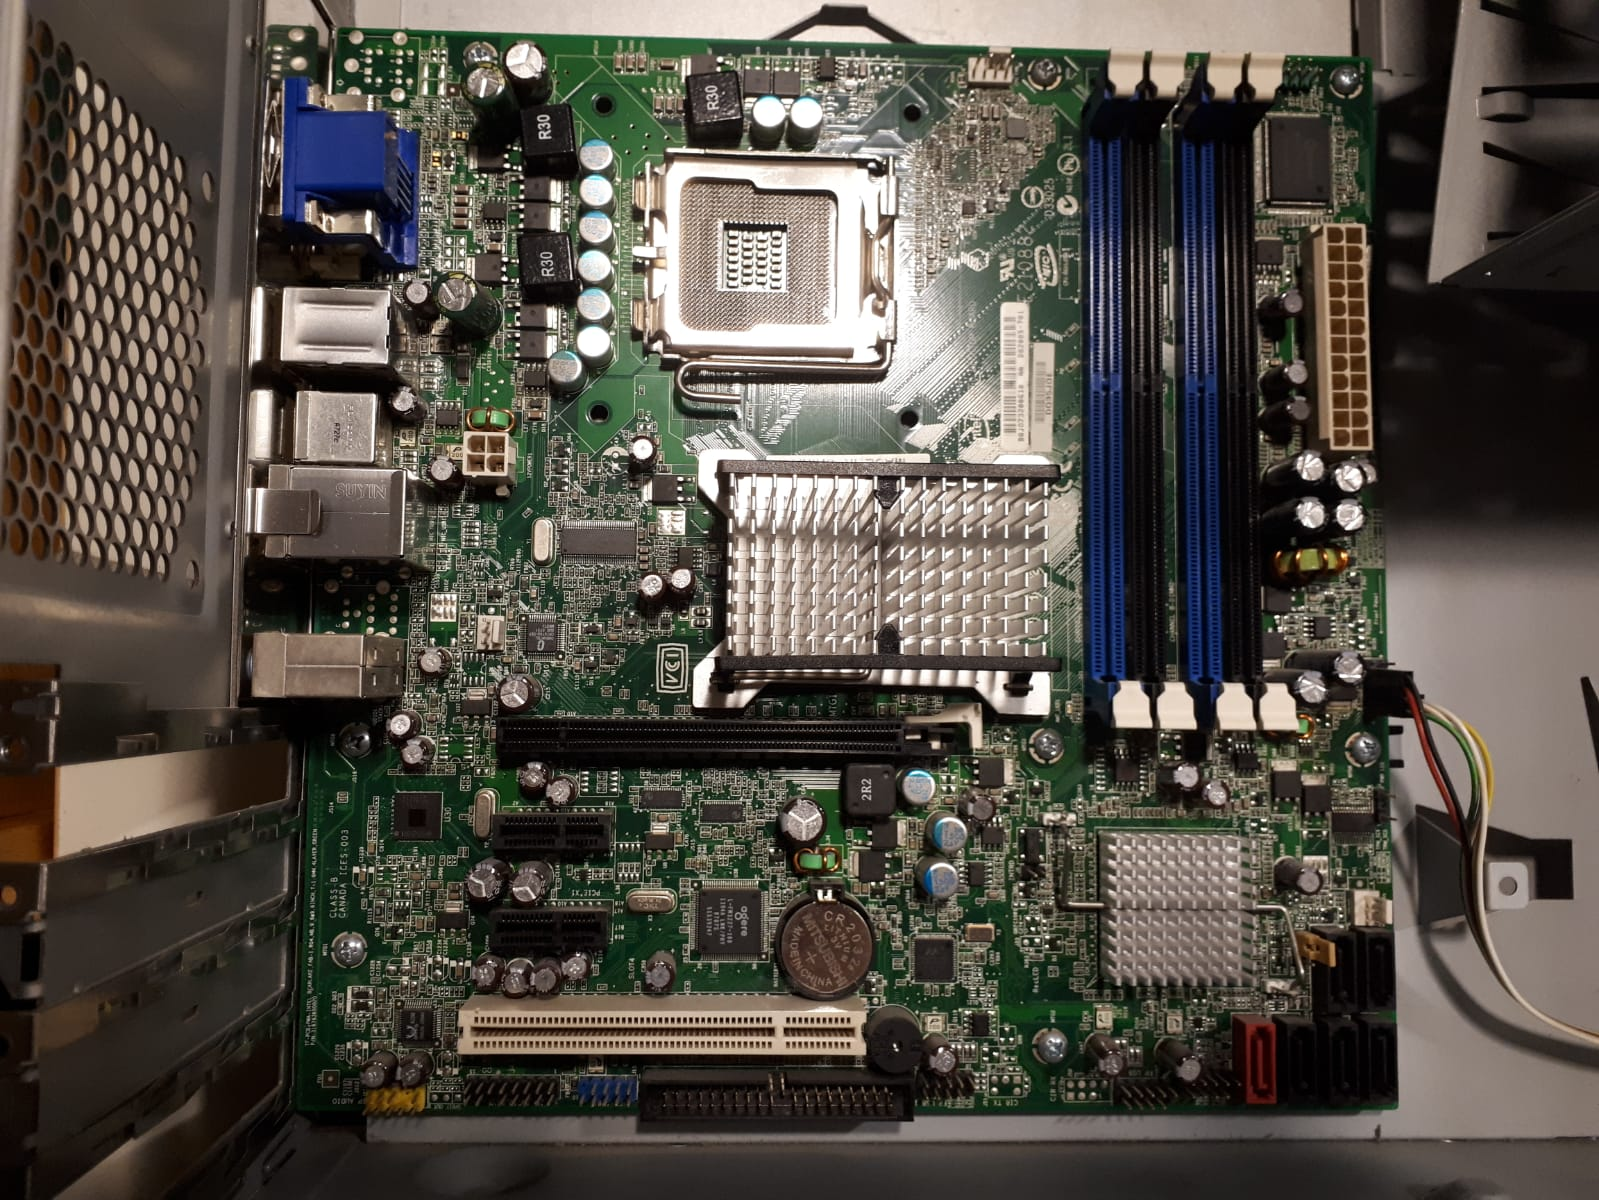
\includegraphics[scale=0.1]{img/mainboard.jpeg}
        \end{columns}
    \end{frame}

	\section{Things to know about Connectors}
    \begin{frame}{Things to know about Connectors}
        \begin{columns}
            \column{0.55\textwidth}
                \begin{itemize}
                    \item most connectors have notches, etc to prevent wrong installation \ra general rule: force = wrong
                    \item external vs internal connectors \ra the latter are  usually much more fragile
                \end{itemize}
            \column{0.45\textwidth}
                \center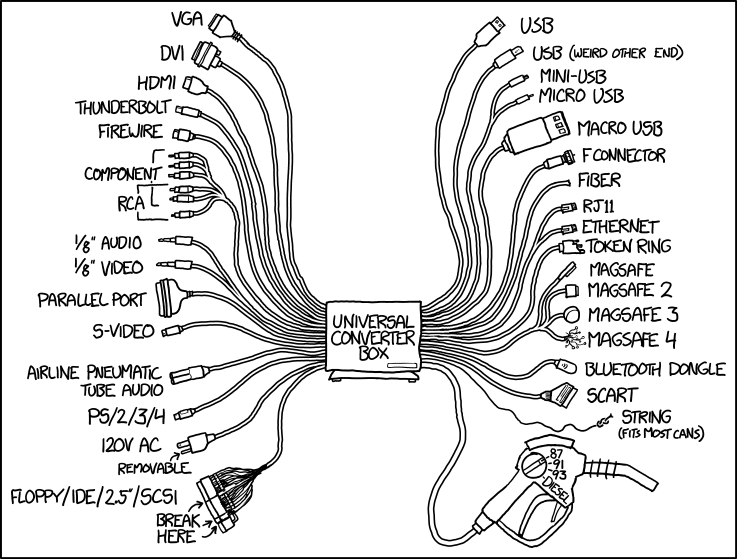
\includegraphics[scale=0.25]{img/connectors.png}
                \center\tiny\url{https://imgs.xkcd.com/comics/universal_converter_box.png}
        \end{columns}
    \end{frame}
\end{document}
